% Build with pdflatex; export the resulting page with PyMuPDF.
% The two parallelograms lie in one fixed Euclidean lattice.
\documentclass[tikz,border=12pt]{standalone}
\usepackage[T1]{fontenc}
\usepackage{lmodern,amsmath}
\usetikzlibrary{arrows.meta,calc}
\definecolor{ink}{HTML}{183444}
\definecolor{blue}{HTML}{1B6780}
\definecolor{amber}{HTML}{AD601A}
\definecolor{teal}{HTML}{26756A}
\begin{document}
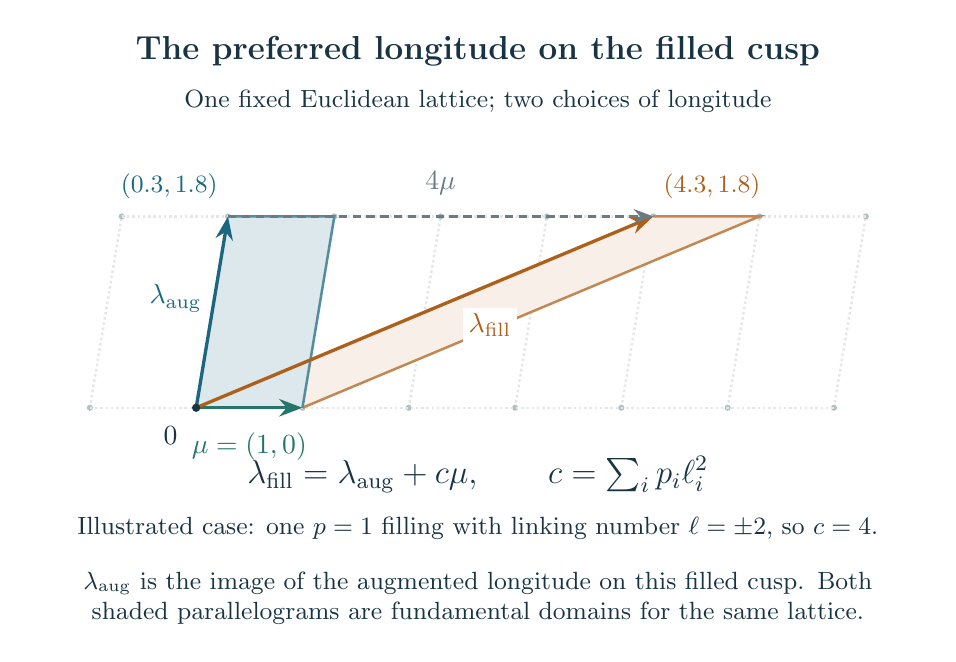
\begin{tikzpicture}[x=1.35cm,y=1.35cm,font=\sffamily,
  text=ink,>=Stealth,line width=.9pt]
  \node[font=\large\bfseries] at (2.65,3.35)
    {The preferred longitude on the filled cusp};
  \node[font=\small,align=center] at (2.65,2.88)
    {One fixed Euclidean lattice; two choices of longitude};

  \coordinate (O) at (0,0);
  \coordinate (M) at (1,0);
  \coordinate (L) at (.3,1.8);
  \coordinate (LM) at (1.3,1.8);
  \coordinate (F) at (4.3,1.8);
  \coordinate (FM) at (5.3,1.8);
  \foreach \j in {-1,0,1,2,3,4,5,6} {
    \draw[ink!12,densely dotted] (\j,0)--({\j+.3},1.8);
    \fill[ink!32] (\j,0) circle (1.1pt);
    \fill[ink!32] ({\j+.3},1.8) circle (1.1pt);
  }
  \draw[ink!12,densely dotted] (-1,0)--(6,0);
  \draw[ink!12,densely dotted] (-.7,1.8)--(6.3,1.8);
  \fill[amber!10] (O)--(M)--(FM)--(F)--cycle;
  \fill[blue!15] (O)--(M)--(LM)--(L)--cycle;
  \draw[amber!75] (M)--(FM)--(F);
  \draw[blue!75] (M)--(LM)--(L);
  \draw[teal,very thick,->] (O)--node[below=5pt]{$\mu=(1,0)$}(M);
  \draw[blue,very thick,->] (O)--(L);
  \draw[amber,very thick,->] (O)--(F);
  \draw[ink!65,densely dashed,->] (L)--node[above=4pt]{$4\mu$}(F);
  \node[blue,anchor=east,align=right] at (.15,1.03)
    {$\lambda_{\mathrm{aug}}$};
  \node[amber,anchor=north west,fill=white,inner sep=2pt]
    at (2.5,.95) {$\lambda_{\mathrm{fill}}$};
  \node[blue,anchor=south east,font=\small] at (.3,1.87)
    {$(0.3,1.8)$};
  \node[amber,anchor=south west,font=\small] at (4.3,1.87)
    {$(4.3,1.8)$};
  \fill[ink] (O) circle (1.5pt);
  \node[below left=3pt] at (O) {$0$};

  \node[font=\large] at (2.65,-.63)
    {$\lambda_{\mathrm{fill}}=\lambda_{\mathrm{aug}}+c\mu,
      \qquad c=\sum_i p_i\ell_i^2$};
  \node[font=\small,align=center] at (2.65,-1.13)
    {Illustrated case: one $p=1$ filling with linking number $\ell=\pm2$,
     so $c=4$.};
  \node[font=\small,align=center,text width=11.2cm] at (2.65,-1.79)
    {$\lambda_{\mathrm{aug}}$ is the image of the augmented longitude
     on this filled cusp. Both shaded parallelograms are fundamental
     domains for the same lattice.};
\end{tikzpicture}
\end{document}
